\subsection{Sonstiges}

\begin{figure}[h]
    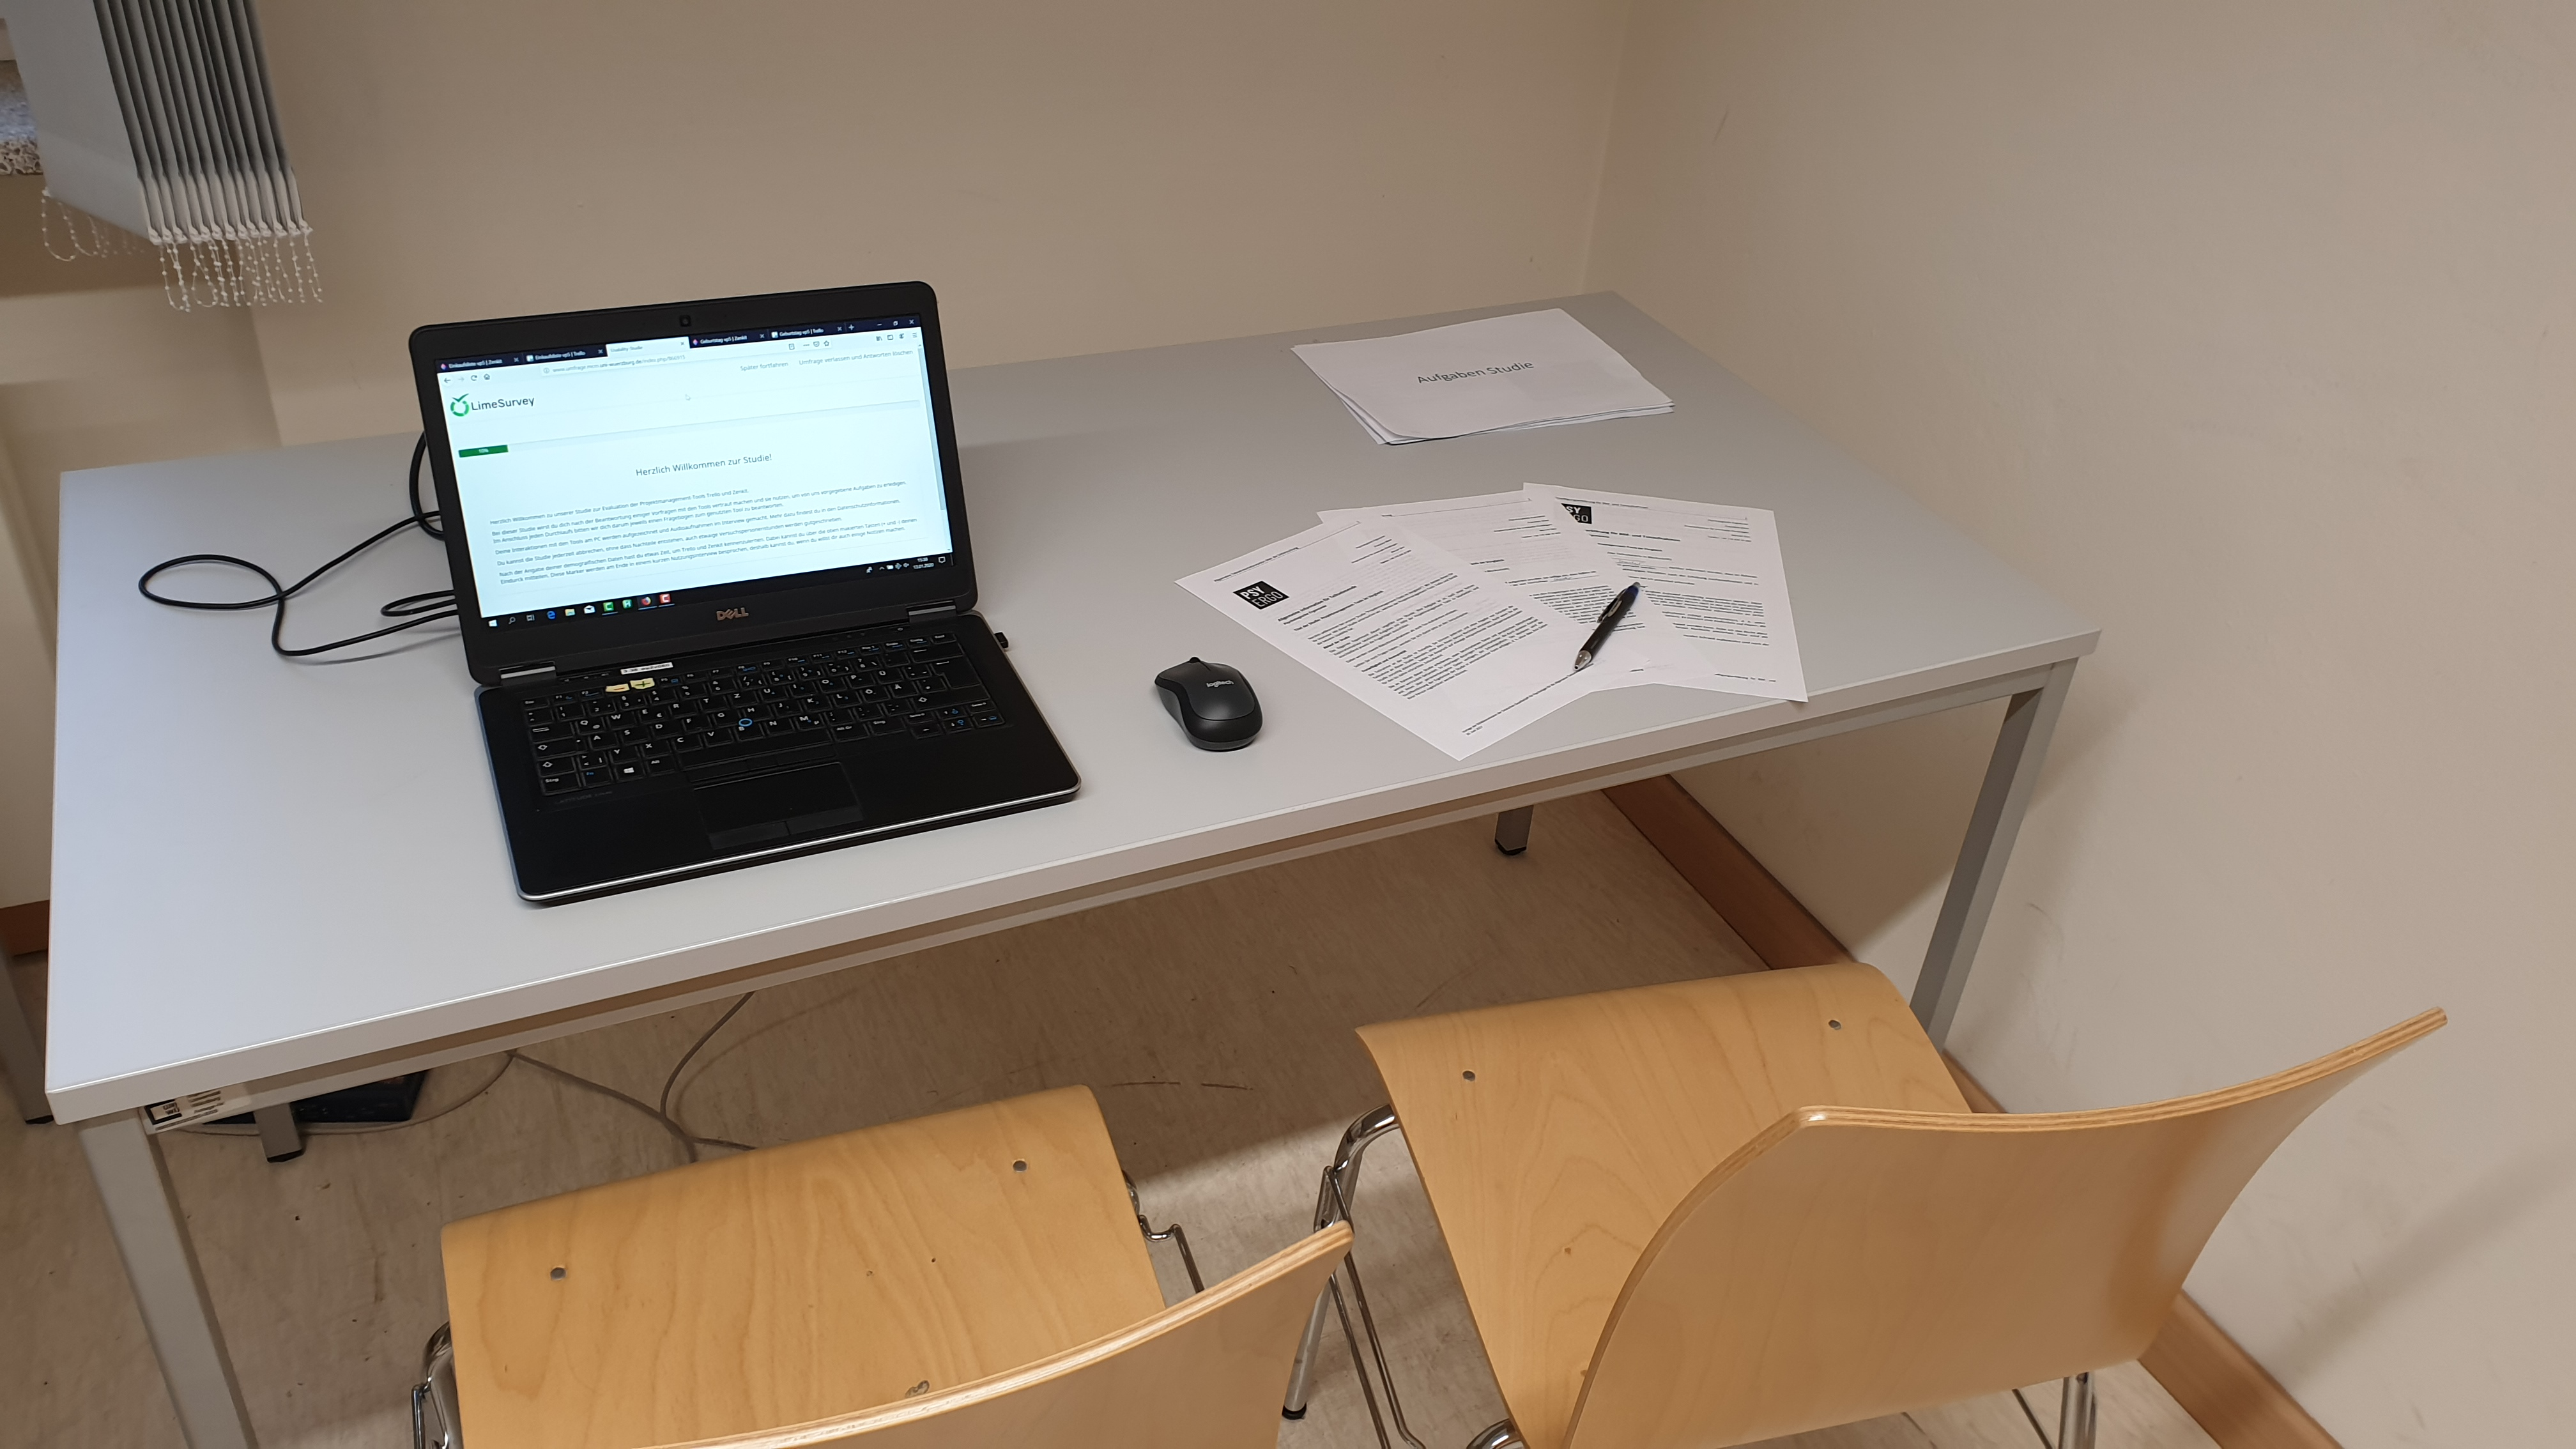
\includegraphics[width=0.9\textwidth]{images/Sonstiges/Studie-Aufbau.jpg}
    \centering
    \caption{Versuchssituation, wie sie die Versuchsperson zu Beginn der Studie vorfand}
    \label{fig:aufbau}
\end{figure}

\begin{figure}[h]
    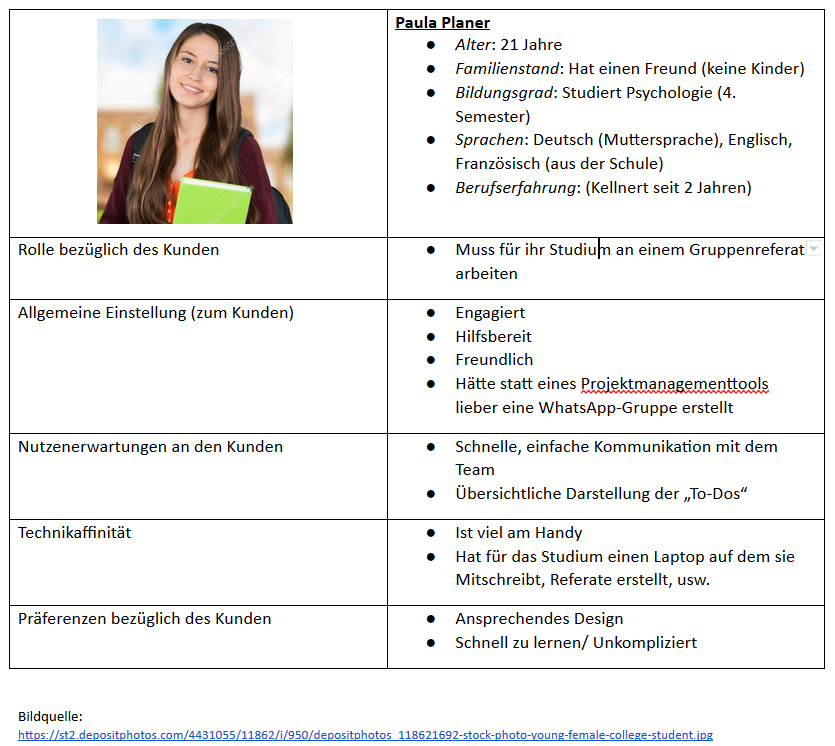
\includegraphics[width=0.7\textwidth]{images/Sonstiges/persona.PNG}
    \centering
    \caption{Persona, die als Hintergrund bzw. Ausgangspunkt für die Heuristische Evaluation genutzt wurde.}
    \label{fig:persona}
\end{figure}

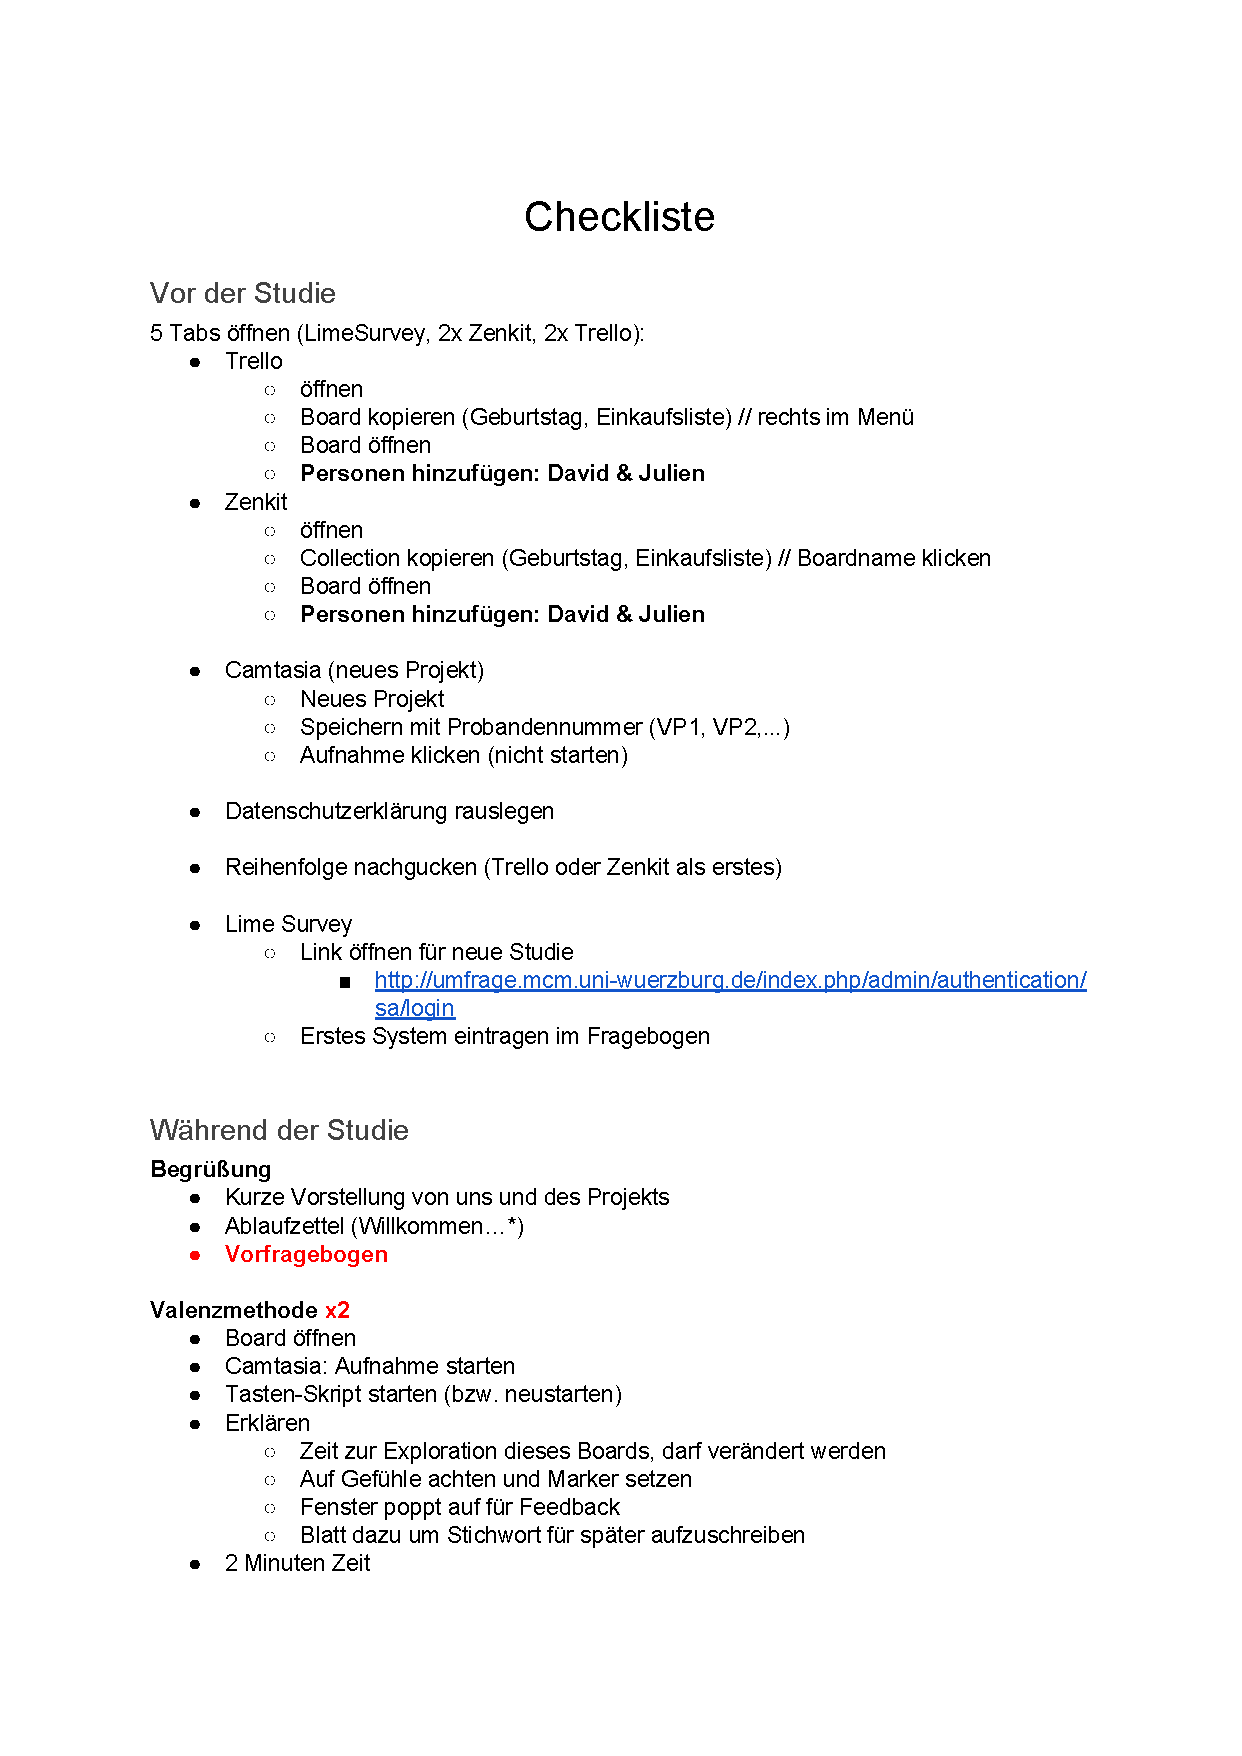
\includepdf[pages=-,scale=.8, pagecommand={}]{images/pdf/Checkliste.pdf}

\begin{figure}[h]
    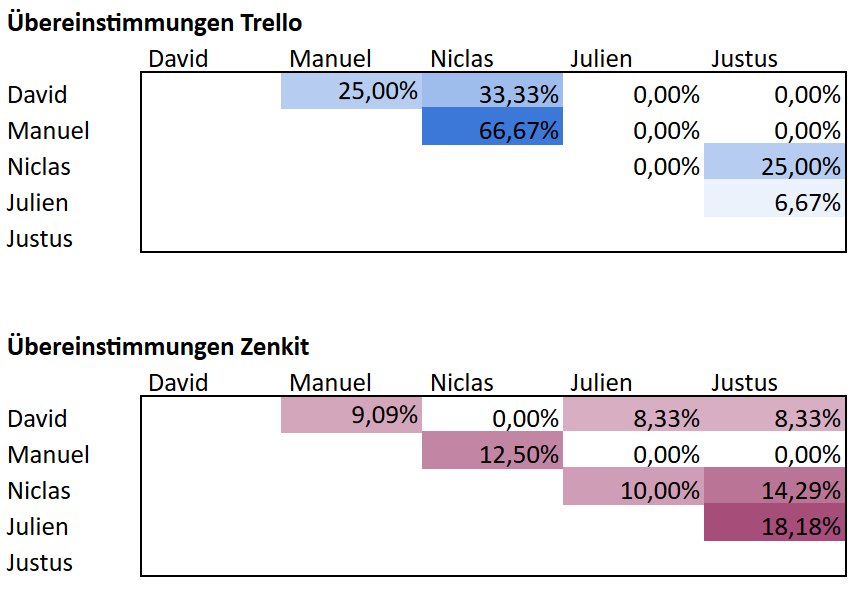
\includegraphics[width=0.7\textwidth]{images/Statistiken/uebereinstimmungen.PNG}
    \centering
    \caption{Übereinstimmungen zwischen den Evaluatoren bezüglich der gefundenen Probleme bei der Heuristischen Evaluation. Berechnet als Anteil der Probleme, die von beiden Evaluatoren gefunden wurden.}
    \label{fig:uebereinstimmungen}
\end{figure}

\begin{figure}[h]
    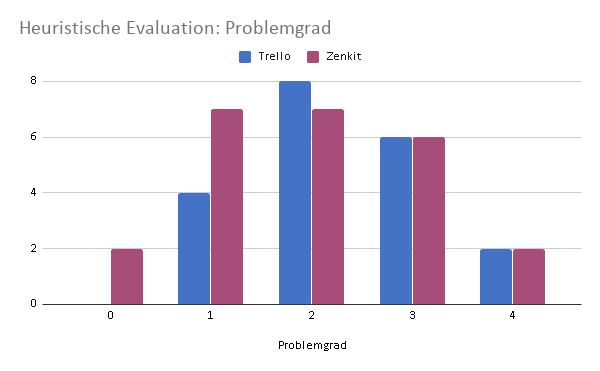
\includegraphics[width=0.8\textwidth]{images/Statistiken/problemgrad.png}
    \caption{Verteilung der gefundenen Probleme der Heuristischen Evaluation nach Problemgrad}
    \label{fig:gefundene_probleme}
\end{figure}

\begin{figure}[H]
    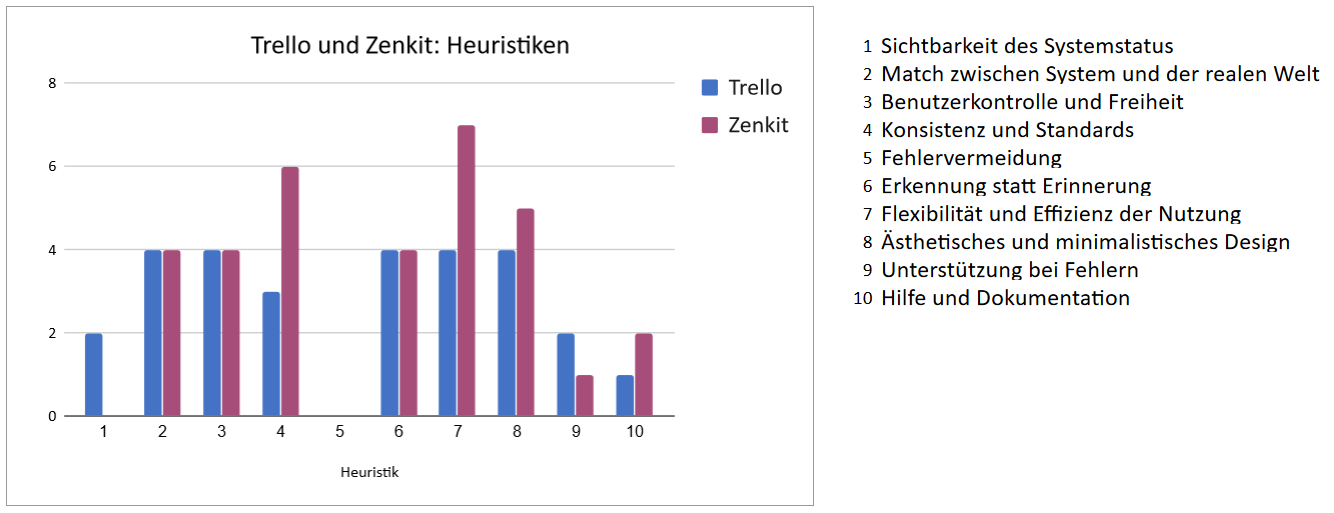
\includegraphics[width=0.9\textwidth]{images/Statistiken/probleme_heuristiken_neu.png}
    \centering
    \caption{Anzahl der gefundenen Probleme pro Heuristik}
    \label{fig:heuristik_probleme}
\end{figure}

\begin{figure}[h]
    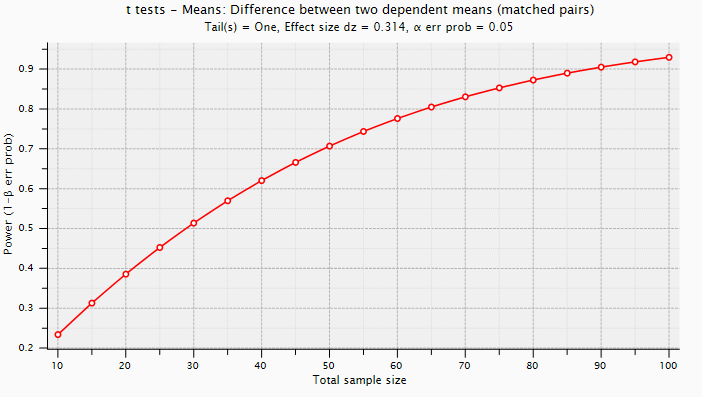
\includegraphics[width=0.7\textwidth]{images/Statistiken/powertlx.PNG}
    \centering
    \caption{Die Teststärke als Funktion der Stichprobengröße des NASA-TLX-Anstrengung Tests}
    \label{fig:powertlx}
\end{figure}


\begin{figure}[h]
    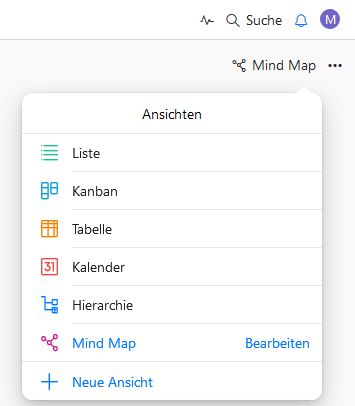
\includegraphics[width=0.4\textwidth]{images/UI/zenkit_ansichten.PNG}
    \centering
    \caption{Auswahl der möglichen Ansichten Zenkits neben des Kanban Standards}
    \label{fig:views}
\end{figure}

\FloatBarrier
